\section{リリースについて}
最終成果発表会で得られたレビューをもとに第4サイクルについて改善を行った後、2月頃までのリリースを目標としている。この時期にリリース目標を設定した理由としては、3月に北海道新幹線が開業することが挙げられる。観光客が最も訪れると予想される開業直後に間に合うようリリース準備を進めていく予定だ。今後の作業としては、まずレビューをもとに機能の拡張やUIの再設計を行い、並行して既知のバグの修正を行っていく。これらが完了し次第、App Storeへリリースする。また、リリース後にも定期的なメンテナンスを行っていくほか、季節ごとのコンテンツの追加などの案も検討されている。なお、リリース後のメンテナンスについては、指導教員より最低でも2年間は継続することが望ましいと指導を受けている。
\begin{figure}[htbp]
  \begin{center}
    \begin{tabular}{c}

      % 1
      \begin{minipage}{0.7\hsize}
        \begin{center}
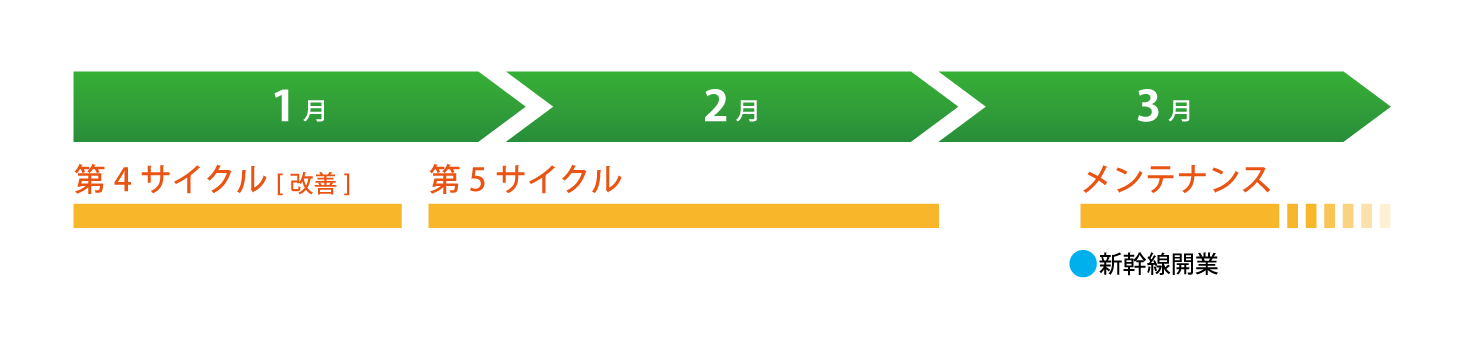
\includegraphics[width=8cm, bb=0 0 1478 338]{release-1.png}
       
        \end{center}
      \end{minipage}

    \end{tabular}
    \caption{今後の予定}
    \label{fig:lena}
  \end{center}
\end{figure}
\bunseki{横山翔栄}